\paperchapter{December 2021}{23 January 2022}{A}{50}{15th GSET}
\keytable{\kcell{1}{A} & \kcell{2}{A} & \kcell{3}{B} & \kcell{4}{B} & \kcell{5}{C} & \kcell{6}{B} & \kcell{7}{D} & \kcell{8}{B} & \kcell{9}{C} & \kcell{10}{A} \\
\kcell{11}{B} & \kcell{12}{B} & \kcell{13}{B} & \kcell{14}{B} & \kcell{15}{A} & \kcell{16}{B} & \kcell{17}{A} & \kcell{18}{C} & \kcell{19}{C} & \kcell{20}{B} \\
\kcell{21}{B} & \kcell{22}{A} & \kcell{23}{D} & \kcell{24}{D} & \kcell{25}{D} & \kcell{26}{C} & \kcell{27}{B} & \kcell{28}{A} & \kcell{29}{B} & \kcell{30}{D} \\
\kcell{31}{B} & \kcell{32}{C} & \kcell{33}{C} & \kcell{34}{D} & \kcell{35}{C} & \kcell{36}{A} & \kcell{37}{D} & \kcell{38}{D} & \kcell{39}{C} & \kcell{40}{C} \\
\kcell{41}{C} & \kcell{42}{D} & \kcell{43}{D} & \kcell{44}{B} & \kcell{45}{D} & \kcell{46}{C} & \kcell{47}{C} & \kcell{48}{C} & \kcell{49}{A} & \kcell{50}{D}}
\begin{question}{1}
{Identify which of the following steps are carried out for constant comparison in grounded theory research?\par}
\optsone{Data collection, note taking, coding and memoing}{Data collection, data reduction, data display, conclusion drawing and verification}{Data collection, axial coding, categorization and narrative description}{Data collection, contrasting, comparing and generating themes and patterns}
\answer{A}{Data collection, note taking, coding and memoing}
\begin{explain}
In \textbf{grounded theory} (Glaser \& Strauss, 1967) the \emph{constant comparative method} runs as a cycle. The researcher \textbf{collects data}, takes \textbf{field notes}, \textbf{codes} the data (open, axial and selective coding) and writes \textbf{memos}, comparing each new piece of data with earlier codes and categories until theoretical saturation is reached.
\why{(B) is Miles \& Huberman's interactive model of qualitative analysis; (C) mixes coding with narrative description; (D) describes generic thematic analysis.}
\end{explain}
\end{question}

\begin{question}{2}
{Which of the following is common in all true experimental and Quasi experimental designs?\par}
\optstwo{Control group}{Randomization}{Pre-testing and post-testing}{Pre-testing}
\answer{A}{Control group}
\begin{explain}
True experimental designs always have a \emph{control group} and random assignment. Quasi-experimental designs (e.g.\ the non-equivalent control group design) \emph{lack randomization} but still compare treated units with a control or comparison group. The common element, as per the official key, is the \textbf{control group}.
\why{Randomization is absent in quasi-experiments, and pre-testing is not used in every design (e.g.\ the post-test-only control group design).}
\end{explain}
\end{question}

\begin{question}{3}
{Find the wrong term in the letter-number series given below.\newline G4T, J10R, M20P, P43N, S90L\par}
\optsfour{G4T}{J10R}{M20P}{P43N}
\answer{B}{J10R}
\begin{explain}
\begin{itemize}
\item Letters: G, J, M, P, S (+3) and T, R, P, N, L ($-2$) are both regular.
\item Numbers should follow $\times2+1, \times2+2, \times2+3, \times2+4$: $4\rightarrow\mathbf{9}\rightarrow20\rightarrow43\rightarrow90$.
\end{itemize}
The second term should be J\textbf{9}R, so \textbf{J10R} is wrong.
\end{explain}
\end{question}

\begin{question}{4}
{A cube whose each corner is named as A, B, C, D, F, G and H is segmented into 27 equal tiny cubes. Before dividing the cube, each face of its varnished with different colours. How many tiny cubes will be formed having more than one colour?\par}
\optsfour{64}{20}{55}{53}
\answer{B}{20}
\begin{explain}
A cube cut into $3\times3\times3=27$ small cubes, with each face painted a different colour:
\begin{itemize}
\item corner cubes have 3 colours: \textbf{8};
\item edge (middle-of-edge) cubes have 2 colours: $12\times(3-2)=\mathbf{12}$;
\item face-centre cubes have 1 colour: 6; the central cube has none: 1.
\end{itemize}
Cubes with more than one colour $=8+12=\mathbf{20}$.
\end{explain}
\end{question}

\begin{question}{5}
{Which of the following is not true in relation to 'SWAYAM'?\par}
\optsone{It is Sanskrit acronym that stands for 'Study Webs of Active-Learning for Young Aspiring Minds'}{It is an Indian Massive Open Online Course (MOOC) platform}{It has been developed jointly by MHRD (now MoE) and UGC with the help of Infosys}{It is under 'Digital India' to give a coordinated stage and free entry to web courses covering all advance education and skill sector courses}
\answer{C}{It has been developed jointly by MHRD (now MoE) and UGC with the help of Infosys}
\begin{explain}
SWAYAM was developed by \textbf{MHRD (now MoE) and AICTE with the help of Microsoft}, not by UGC with Infosys. So statement (C) is not true. The other statements are correct: SWAYAM stands for \emph{Study Webs of Active-Learning for Young Aspiring Minds}, is India's MOOC platform, and was launched under Digital India.
\end{explain}
\end{question}

\begin{question}{6}
{Which of the following are game based learning platforms?\newline a. Kahoot\newline b. Socrative\newline c. Quizizz\newline d. e-PG Pathshala\newline e. Edmodo\par}
\optsfour{e, d and b}{a, b and c}{a, c and d}{c, e and a}
\answer{B}{a, b and c}
\begin{explain}
\textbf{Kahoot}, \textbf{Socrative} and \textbf{Quizizz} are game-based, quiz-style learning and assessment platforms with points, leaderboards and timers.
\why{e-PG Pathshala is a UGC/INFLIBNET e-content repository for postgraduate subjects; Edmodo is a learning-management and social-classroom platform.}
\end{explain}
\end{question}

\begin{question}{7}
{In a certain relationship\newline $M/N$ means M is daughter of N\newline $M+N$ means M is father of N\newline M-N means M is mother of N\newline Answer the following question based on data above.\newline In the pattern $F^{*}G/H-I$, how is I related to G?\par}
\optsfour{Mother}{Sister}{Niece}{No relation}
\answer{D}{No relation}
\begin{explain}
$G/H$: G is the daughter of H. $H-I$: H is the mother of I. So I is a child of H, i.e.\ a sibling of G. The symbol ``$*$'' in $F*G$ is not defined in the code, and I's gender is not given, so ``Sister'' cannot be concluded. Mother and niece are clearly wrong. The official key gives \textbf{(D) No relation} (i.e.\ none of the definite relations offered can be established).
\end{explain}
\end{question}

\begin{question}{8}
{In the following figure triangle represents 'girls', square 'players' and circle 'coach'. Which part of the diagram represents the girls are player but not coach?\par}
\qfigure{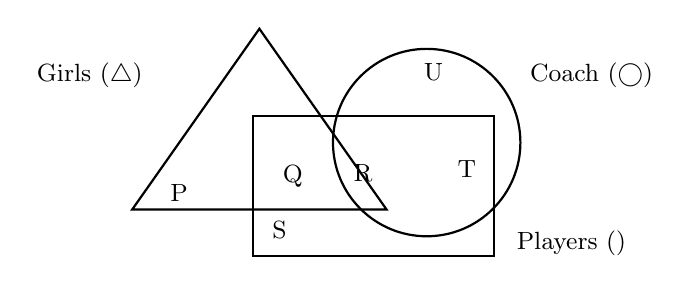
\begin{tikzpicture}[scale=0.85,font=\small]
\draw[thick] (-1.6,-0.5) -- (0.3,2.2) -- (2.2,-0.5) -- cycle;
\draw[thick] (0.2,-1.2) rectangle (3.8,0.9);
\draw[thick] (2.8,0.5) circle (1.4);
\node at (-0.9,-0.25) {P}; \node at (0.8,0) {Q}; \node at (1.85,0.05) {R}; \node at (0.6,-0.8) {S}; \node at (2.9,1.55) {U}; \node at (3.4,0.1) {T};
\node[left] at (-1.3,1.5) {Girls ($\triangle$)}; \node[right] at (4.2,1.5) {Coach ($\bigcirc$)}; \node[right] at (4.0,-1.0) {Players ($\square$)};
\end{tikzpicture}}
\optsfour{P}{Q}{R}{S}
\answer{B}{Q}
\begin{explain}
Girls who are players but not coaches lie \textbf{inside the triangle and inside the square but outside the circle}. That region is \textbf{Q}.
\why{P = girls only; R = girls who are players \emph{and} coaches; S = players only (not girls).}
\end{explain}
\end{question}

\begin{question}{9}
{If a student ask you a question whose answer is not known to you, then\newline 1. Give this question as a homework and start teaching.\newline 2. Tell him this question will be answered the next day.\newline 3. Ask him to come later and then send him to library.\newline 4. After the class you will go to library and try to find the answer.\newline 5. Appreciate the question and accept that you don't have information right now.\par}
\optsfour{1, 2 and 4}{3, 4 and 5}{2, 4 and 5}{2, 3 and 5}
\answer{C}{2, 4 and 5}
\begin{explain}
A good teacher is honest and a model learner: \textbf{appreciates the question and admits not knowing (5)}, \textbf{consults the library after class (4)} and \textbf{answers it the next day (2)}. Giving it as homework to hide ignorance (1) or sending the student away (3) is inappropriate. The answer is 2, 4 and 5.
\end{explain}
\end{question}

\begin{question}{10}
{Which of the following is most applicable to split half method of finding reliability ?\par}
\optsone{It shows the internal consistency of the test}{It shows the internal consistency of half of the test}{It can be used for tests having both subjective and objective type questions}{It can be used for tests with any number of items}
\answer{A}{It shows the internal consistency of the test}
\begin{explain}
In the \textbf{split-half method} one test is divided into two comparable halves (e.g.\ odd and even items), the two half-scores are correlated, and the result is stepped up with the Spearman--Brown formula $r_{tt}=\frac{2r_{hh}}{1+r_{hh}}$. It measures the \textbf{internal consistency of the whole test}.
\why{It needs a sufficiently large, even number of homogeneous items that can be split, and is unsuitable for speed tests.}
\end{explain}
\end{question}

\begin{question}{11}
{Match the List--I with List--II and choose the correct option given below.\\[2pt]
\begin{tabular}{@{}p{0.44\linewidth}p{0.5\linewidth}@{}}
\textbf{List--I} & \textbf{List--II}\\
1. National Institute of Educational Planning and Administration (NIEPA) & a. Deemed to be a University, 1964, under Section 3 of UGC Act, 1956\\
2. Tata Institute of Social Sciences (TISS) & b. A Central University and An Institution of National Importance\\
3. Mahatma Gandhi Antarrashtriya Hindi Vishwavidyalaya (MGAHV) & c. A Central University, established by an Act of Parliament, Act No.~3 of 1997\\
4. Visva-Bharati & d. Deemed to be University, 2006, under Section 3 of UGC Act, 1956\\
\end{tabular}\par}
\optstwo{1-b, 2-a, 3-c, 4-d}{1-d, 2-a, 3-c, 4-b}{1-b, 2-d, 3-c, 4-a}{1-c, 2-b, 3-d, 4-a}
\answer{B}{1-d, 2-a, 3-c, 4-b}
\begin{explain}
\begin{itemize}
\item \textbf{NIEPA} (now NIEPA, New Delhi) became a deemed university in \textbf{2006}, so 1-d.
\item \textbf{TISS}, Mumbai (founded 1936) was declared deemed in \textbf{1964}, so 2-a.
\item \textbf{MGAHV}, Wardha was established by \textbf{Act No.~3 of 1997}, so 3-c.
\item \textbf{Visva-Bharati}, Santiniketan (founded by Tagore) is a central university and an \textbf{institution of national importance} (Visva-Bharati Act, 1951), so 4-b.
\end{itemize}
\end{explain}
\end{question}

\begin{question}{12}
{Which of the following is not an independent vertical of one umbrella institution i.e. Higher Education Commission of India (HECI) as proposed in NEP 2020?\par}
\optsone{National Higher Education Regulatory Council (NHERC)}{University Education Council (UEC)}{General Education Council (GEC)}{Higher Education Grants Council (HEGC)}
\answer{B}{University Education Council (UEC)}
\begin{explain}
NEP~2020 proposes the \textbf{Higher Education Commission of India (HECI)} with four independent verticals:
\begin{enumerate}
\item \textbf{NHERC}, the National Higher Education Regulatory Council (regulation);
\item \textbf{NAC}, the National Accreditation Council (accreditation);
\item \textbf{HEGC}, the Higher Education Grants Council (funding);
\item \textbf{GEC}, the General Education Council (standard setting).
\end{enumerate}
A ``University Education Council'' is not one of them.
\end{explain}
\end{question}

\begin{question}{13}
{In a certain code $E=P$, $Z=C,$ $N=O$ $K=B$, $C=Q$ $A=X$ $R=H$, $B=R.$ How will BREAK be written in the same code?\par}
\optsfour{RHPBX}{RHPXB}{RHPXC}{ROPXB}
\answer{B}{RHPXB}
\begin{explain}
Using the given code: B$\rightarrow$R, R$\rightarrow$H, E$\rightarrow$P, A$\rightarrow$X, K$\rightarrow$B.
BREAK $\rightarrow$ \textbf{RHPXB}.
\end{explain}
\end{question}

\begin{question}{14}
{A and B travels from point P to Q at $17~km/hr$ and $19~km/hr$. respectively. P is 72 km away from Q. B reaches Q first and returns immediately and meets A at R. What is the distance between Q and R?\par}
\optsfour{10 km}{4 km}{15 km}{36 km}
\answer{B}{4 km}
\begin{explain}
Until they meet, A and B together cover $PQ+QR+PR=2\times72=144$ km.
\[t=\frac{144}{17+19}=4\text{ h};\quad\text{B covers }19\times4=76\text{ km}=72+QR\ \Rightarrow\ QR=\mathbf{4\ km}\]
\end{explain}
\end{question}

\begin{question}{15}
{Match List - I with List - II and select the correct option given below.\par\smallskip\begin{tabularx}{\linewidth}{@{}>{\raggedright\arraybackslash}X>{\raggedright\arraybackslash}X@{}}\toprule
\textbf{List-I (Software)} & \textbf{List - II (Application)}\\\midrule
1. Mendeley & a. Quantitative data analysis\\
2. SPSS & b. Reference manager\\
3. Turnitin & c. Plagiarism check\\
4. Nvivo & d. Qualitative data analysis\\
\bottomrule\end{tabularx}\par\smallskip
\par}
\optstwo{1-b, 2-a, 3-c, 4-d}{1-d, 2-a, 3-c, 4-b}{1-c, 2-a, 3-b, 4-d}{1-c, 2-a, 3-d, 4-b}
\answer{A}{1-b, 2-a, 3-c, 4-d}
\begin{explain}
Mendeley is a \textbf{reference manager} (1-b); SPSS does \textbf{quantitative} analysis (2-a); Turnitin checks \textbf{plagiarism} (3-c); NVivo does \textbf{qualitative} analysis (4-d).
\end{explain}
\end{question}

\begin{question}{16}
{Which of the following statement/s is/are correct?\newline a. For the sequence of integers represented in binary 00111, 01001, 01011, P.\ldots{} the next integer P would be represented as 011101.\newline b. A byte is a binary number consisting of exactly 8 bits.\newline Choose the correct option:\par}
\optstwo{a only}{b only}{both a and b}{neither a nor b}
\answer{B}{b only}
\begin{explain}
(a) $00111=7$, $01001=9$, $01011=11$: odd numbers, so next is $13=\mathbf{01101}$, not $011101$ ($=29$). Statement (a) is false.
(b) A byte is exactly 8 bits. Statement (b) is true. So \textbf{b only}.
\end{explain}
\end{question}

\begin{question}{17}
{Study the chart and answer the question. The pie chart given here represents the domestic expenditure of a family in percent. If the total monthly income of the family is Rs.~55,660/-, the annual savings in the form of PF would be (in nearest Rs.)\par}
\qfigure{\begin{tikzpicture}[scale=1]
\pie[radius=1.3,text=pin,color={brand!15,brand!35,brand!10,brand!45,brand!25,brand!5},font=\tiny]{9/Medical,13/PF,23/Food,18/House Rent,12/Entertain.,25/Child Edu.}
\end{tikzpicture}}
\optsfour{86830}{86155}{96830}{76830}
\answer{A}{86830}
\begin{explain}
Monthly PF $=13\%\times55{,}660=7{,}235.80$.
Annual PF $=7{,}235.80\times12=86{,}829.6\approx$ \textbf{Rs.~86,830}.
\end{explain}
\end{question}

\begin{question}{18}
{Choose the graph that best fits with this statement: "This car has excellent acceleration".\par}
\optsfour{\tikz[baseline=3mm,scale=0.45]{\draw[->](0,0)--(2.6,0);\draw[->](0,0)--(0,1.6);\draw[thick,brand](0,1)--(1.8,1);}}{\tikz[baseline=3mm,scale=0.45]{\draw[->](0,0)--(2.6,0);\draw[->](0,0)--(0,1.6);\draw[thick,brand](0,0.8) .. controls (1.2,0.8) and (1.8,1) .. (2,1.5);}}{\tikz[baseline=3mm,scale=0.45]{\draw[->](0,0)--(2.6,0);\draw[->](0,0)--(0,1.6);\draw[thick,brand](0,0)--(1.9,1.5);}}{\tikz[baseline=3mm,scale=0.45]{\draw[->](0,0)--(2.6,0);\draw[->](0,0)--(0,1.6);\draw[thick,brand](0,0.6) .. controls (0.4,1.3) and (0.6,1.4) .. (0.9,0.9) .. controls (1.1,0.6) and (1.3,0.9) .. (1.6,0.95) -- (2.3,0.95);}}
\answer{C}{\tikz[baseline=3mm,scale=0.45]{\draw[->](0,0)--(2.6,0);\draw[->](0,0)--(0,1.6);\draw[thick,brand](0,0)--(1.9,1.5);}}
\begin{explain}
Plotting speed against time, excellent acceleration means the speed rises \textbf{quickly and steadily from rest}: a straight, steep line through the origin, as in graph (C).
\why{(A) shows constant speed (no acceleration); (B) starts with an almost flat curve (sluggish at first); (D) rises, falls and levels off.}
\end{explain}
\end{question}

\begin{question}{19}
{A group of students of your class face problem in learning, you want to identify the deficiencies and difficulties of the learner, which evaluation would you choose?\par}
\optstwo{Formative evaluation}{Summative evaluation}{Diagnostic evaluation}{Qualitative evaluation}
\answer{C}{Diagnostic evaluation}
\begin{explain}
\textbf{Diagnostic evaluation} identifies the specific learning difficulties and their causes, so that remedial teaching can follow.
\why{Formative evaluation monitors progress during teaching; summative evaluation certifies achievement at the end.}
\end{explain}
\end{question}

\begin{question}{20}
{What should be done to ensure optimum growth of the slow learner?\newline 1. They should be treated like others, they will grow themself.\newline 2. They should be given challenging task as per their level in the area of their interest.\newline 3. They should be left at their own.\newline 4. They should get sufficient resources.\newline 5. Regular activities regarding diagnosis and remedy.\par}
\optsfour{1, 3 and 5}{2, 4 and 5}{2, 3 and 4}{3, 4 and 5}
\answer{B}{2, 4 and 5}
\begin{explain}
Slow learners need \textbf{tasks matched to their level and interests (2)}, \textbf{sufficient resources (4)} and \textbf{regular diagnosis and remediation (5)}. Treating them like everyone else or leaving them on their own (1, 3) neglects their needs. The answer is 2, 4 and 5.
\end{explain}
\end{question}

\begin{question}{21}
{Which of the following is a lead agency for 'Education for Sustainable Development'?\par}
\optstwo{Brundtland Commission}{UNESCO}{UNDP}{UNICEF}
\answer{B}{UNESCO}
\begin{explain}
\textbf{UNESCO} is the lead UN agency for \textbf{Education for Sustainable Development (ESD)}. It led the UN Decade of ESD (2005--2014), the Global Action Programme (2015--2019) and now the \emph{ESD for 2030} framework.
\end{explain}
\end{question}

\begin{question}{22}
{The Global Education Development Agenda reflected in the Goal 4 (SDG4) of the 2030 Agenda for Sustainable Development, adopted by India in 2015, seeks to\par}
\optsone{"ensure inclusive and equitable quality education and promote lifelong learning opportunities for all" by 2030}{"ensure inclusive and affordable education and desired learning opportunities for all" by 2030}{"ensure accountable and quality education and promote creative learning opportunities for all" by 2030}{"ensure equity, equality, quality and promote lifelong learning opportunities for all" by 2030}
\answer{A}{"ensure inclusive and equitable quality education and promote lifelong learning opportunities for all" by 2030}
\begin{explain}
SDG~4 reads: ``\textbf{Ensure inclusive and equitable quality education and promote lifelong learning opportunities for all}'' by 2030.
\end{explain}
\end{question}

\begin{question}{23}
{A researcher uses systematic random sampling from a company directory that has 600 employees listed in alphabetical order. If the desired samples size is 30, and the first name to be selected is number 8, which of the following will not be selected?\par}
\optsfour{88}{368}{428}{558}
\answer{D}{558}
\begin{explain}
Interval $k=600/30=20$. The selected numbers are $8, 28, 48, \ldots$, i.e.\ $8+20m$.
$88=8+80$ \checkmark, $368=8+360$ \checkmark, $428=8+420$ \checkmark, but $558-8=550$ is not a multiple of 20. So \textbf{558 is not selected}.
\end{explain}
\end{question}

\begin{question}{24}
{The bar graph given below shows the Foreign Exchange Reserves of a Country (in millions US \$) from 1991-92 to 1998-99. The foreign exchange reserves in 1997-98 was how many times that in 1994-95.\par}
\qfigure{\begin{tikzpicture}
\begin{axis}[ybar,width=10cm,height=4.4cm,bar width=11pt,ymin=0,ymax=5800,
  symbolic x coords={91-92,92-93,93-94,94-95,95-96,96-97,97-98,98-99},xtick=data,
  nodes near coords,every node near coord/.append style={font=\tiny},
  tick label style={font=\scriptsize},ylabel={\scriptsize million US\$},
  axis x line*=bottom,axis y line*=left]
\addplot[fill=brand!70,draw=brand] coordinates {(91-92,2640) (92-93,3720) (93-94,2520) (94-95,3360) (95-96,3120) (96-97,4320) (97-98,5040) (98-99,3120)};
\end{axis}
\end{tikzpicture}}
\optsfour{0.7}{1.2}{1.4}{1.5}
\answer{D}{1.5}
\begin{explain}
\[\frac{\text{Reserves in 1997--98}}{\text{Reserves in 1994--95}}=\frac{5040}{3360}=\mathbf{1.5}\]
\end{explain}
\end{question}

\begin{question}{25}
{Which of the following is not a barrier of the Effective Communication?\par}
\optstwo{Poor ability to listen others}{Lack of transparency and trust}{Cultural and language differences}{Differences in economic status}
\answer{D}{Differences in economic status}
\begin{explain}
Poor listening, lack of trust and transparency, and cultural and language differences all hinder communication. A mere \textbf{difference in economic status} does not by itself prevent effective communication, so it is not a barrier in this list.
\end{explain}
\end{question}

\begin{question}{26}
{What are the major components of effective classroom communication?\newline 1. Sense of Humour\newline 2. Feedback\newline 3. Classroom cleanliness\newline 4. Body Language\newline 5. Safe Environment\par}
\optsfour{1, 2, 3, 4}{2, 3, 4, 5}{1, 2, 4, 5}{1, 3, 4, 5}
\answer{C}{1, 2, 4, 5}
\begin{explain}
Effective classroom communication depends on the teacher's \textbf{sense of humour} (1), continuous \textbf{feedback} (2), appropriate \textbf{body language} (4) and a psychologically \textbf{safe environment} (5). Classroom cleanliness is a physical-hygiene factor, not a component of communication. The answer is 1, 2, 4, 5.
\end{explain}
\end{question}

\begin{question}{27}
{A second commitment period of Kyoto protocol that was agreed to in 2012 to extend the agreement to 2020, known as the\par}
\optstwo{Paris Agreement}{Doha Amendment}{International Solar Alliance}{Environment Protection Act}
\answer{B}{Doha Amendment}
\begin{explain}
The \textbf{Doha Amendment} (COP18, Doha, December 2012) set up the \emph{second commitment period} of the Kyoto Protocol, from 2013 to 2020. (The first period ran 2008--2012.)
\why{The Paris Agreement (2015) is a separate treaty; the International Solar Alliance was launched by India and France in 2015; the Environment Protection Act is India's 1986 law.}
\end{explain}
\end{question}

\begin{question}{28}
{Which of the following Statement is true in relation to Agenda 21 of the Earth Summit in Rio de Janerio, Brazil 1992?\par}
\optsone{It was plan of action to be taken globally, nationally and locally in every area in which human impacts on the environment.}{It was planning for base-plan of Millennium Development Goals.}{It was planning for base-plan of Sustainable Development Goals.}{It was plan of action to be taken globally, nationally, locally in every area of gender disparity and inequality.}
\answer{A}{It was plan of action to be taken globally, nationally and locally in every area in which human impacts on the environment.}
\begin{explain}
\textbf{Agenda 21}, adopted at the Rio Earth Summit (UNCED, 1992), is a comprehensive, non-binding plan of action to be taken \textbf{globally, nationally and locally} by the UN, governments and major groups in \textbf{every area in which humans impact the environment}. The ``21'' refers to the 21st century.
\end{explain}
\end{question}

\begin{question}{29}
{Which of the following research need hypothesis testing?\par}
\optstwo{Historical Research}{Ex-post Facto Research}{Ethnographic Research}{Case Study Research}
\answer{B}{Ex-post Facto Research}
\begin{explain}
\textbf{Ex-post facto (causal-comparative) research} studies cause--effect relations after the fact. It starts from hypotheses about possible causes and \textbf{tests} them statistically.
\why{Historical, ethnographic and case-study research are mostly qualitative and exploratory; they generate hypotheses rather than test them.}
\end{explain}
\end{question}

\begin{question}{30}
{Which of the following idea paved the way for a post-positivist paradigm?\par}
\optsone{Evidence-based reality that can be mathematically interpreted}{Evidence-based reality that can be empirically verified}{Empirical evidence is essential for a posteriori knowledge}{All observation including objective reality is fallible}
\answer{D}{All observation including objective reality is fallible}
\begin{explain}
\textbf{Post-positivism} (Karl Popper and others) holds that all observation is theory-laden and \textbf{fallible}; objective reality exists but can be known only imperfectly and probabilistically. This critique of naive positivism opened the way to post-positivism.
\why{Options (A)--(C) restate \emph{positivist} ideas.}
\end{explain}
\end{question}

\begin{question}{31}
{The price of the sugar rise by 25\%, if a family wants to keep their expenses on sugar the same as earlier, the family will have to decrease its consumption of sugar by\par}
\optsfour{25\%}{20\%}{80\%}{75\%}
\answer{B}{20\%}
\begin{explain}
If the price rises by $r\%$, then to keep the expenditure the same, consumption must fall by
\[\frac{r}{100+r}\times100=\frac{25}{125}\times100=\mathbf{20\%}\]
\end{explain}
\end{question}

\begin{question}{32}
{Consider the example of Anumana given below.\newline I. There is fire in mountain\newline II. Because it has smoke\newline III. Wherever there is a smoke, there is fire\newline Which one of the following expresses Vyapti?\par}
\optstwo{Mountain and fire}{Mountain and smoke}{Fire and smoke}{Perceiver and smoke}
\answer{C}{Fire and smoke}
\begin{explain}
\textbf{Vyapti} is the invariable concomitance between the \emph{hetu} (middle term, \textbf{smoke}) and the \emph{sadhya} (major term, \textbf{fire}): ``wherever there is smoke there is fire''. So Vyapti is expressed by \textbf{fire and smoke}.
\end{explain}
\end{question}

\begin{question}{33}
{Report of Kothari Commission 1964-66, National Policy on Education 1986 and National Education Policy 2020 proposed which of the following share of GDP to be invested on Education?\par}
\optsfour{4.5\% of GDP}{5.0\% of GDP}{6.0\% of GDP}{7.5\% of GDP}
\answer{C}{6.0\% of GDP}
\begin{explain}
The \textbf{Kothari Commission} (1964--66) recommended spending \textbf{6\% of GDP} on education. The NPE 1986 (and its 1992 revision) and \textbf{NEP~2020} reiterated this target.
\end{explain}
\end{question}

\begin{question}{34}
{Which of the following is not a function of National Council for Vocational Education and Training (NCVET)?\par}
\optsone{Grants the recognition to quality awarding bodies}{Grants the recognition to quality assessing agencies}{Regulates the functioning through standardised norms, procedures and continuous quality governance}{Assess and accredit institutions of higher learning to work continuously and improve the quality of education}
\answer{D}{Assess and accredit institutions of higher learning to work continuously and improve the quality of education}
\begin{explain}
The \textbf{NCVET} (set up in 2018 under the Ministry of Skill Development) regulates the vocational education and training ecosystem. It recognises and regulates \emph{awarding bodies} and \emph{assessment agencies} and lays down standardised norms for quality. \textbf{Assessing and accrediting institutions of higher learning} is the job of NAAC, not NCVET.
\end{explain}
\end{question}

\begin{question}{35}
{The distinction between laukika and alaukika is made reference to which one of the following pramanas?\par}
\optstwo{Anumana (Inference)}{Upamana (Comparison)}{Pratyaksa (Perception)}{Sbada (Verbal Testimony)}
\answer{C}{Pratyaksa (Perception)}
\begin{explain}
In Nyaya philosophy, \textbf{Pratyaksha} (perception) is classified as \textbf{laukika} (ordinary perception through sense--object contact) and \textbf{alaukika} (extraordinary perception, namely samanya-lakshana, jnana-lakshana and yogaja).
\end{explain}
\end{question}

\begin{question}{36}
{Find the next term of given series:\newline SEQUENTIAL, EQUENTIAL, EQUENTI \ldots{}?\ldots{} QUEN\par}
\optsfour{QUENTI}{QUENT}{UENTI}{EQUENT}
\answer{A}{QUENTI}
\begin{explain}
Letters are removed alternately from the front (one letter) and from the end (two letters):
\begin{center}
SEQUENTIAL $\xrightarrow{-\text{S}}$ EQUENTIAL $\xrightarrow{-\text{AL}}$ EQUENTI $\xrightarrow{-\text{E}}$ \textbf{QUENTI} $\xrightarrow{-\text{TI}}$ QUEN
\end{center}
\end{explain}
\end{question}

\begin{question}{37}
{Which of the following are related to data mapping?\newline 1. It is a process of matching fields from one databases to another.\newline 2. It enables one to accurately connect sensitive data to the identity of the person associated with it.\newline 3. This reduces the potential for errors, helps standardize data, and makes it easier to understand.\newline 4. Data mapping is a critical element of any data privacy framework.\newline 5. It is related to preparing suitable graphs.\par}
\optsfour{1, 2, 3, 5}{2, 3, 4, 5}{1, 3, 4, 5}{1, 2, 3, 4}
\answer{D}{1, 2, 3, 4}
\begin{explain}
\textbf{Data mapping} matches fields from one database or dataset to another (1). It links sensitive data to the individual it belongs to (2), reduces errors and standardises data (3), and is central to data-privacy compliance such as the GDPR (4). Preparing graphs (5) is data \emph{visualisation}, not data mapping. The answer is 1, 2, 3, 4.
\end{explain}
\end{question}

\begin{question}{38}
{Which of the following is not a Cardinal Philosophy of NMEICT mission?\par}
\optsone{No talent of the country should be allowed to go waste.}{All the services available through the content delivery portal 'SAKSHAT' should be free.}{Freely available material on the web should be used so as to avoid reinventing the wheel.}{Rapid expansion of optical fibre cable network for terrestrial broadband connectivity.}
\answer{D}{Rapid expansion of optical fibre cable network for terrestrial broadband connectivity.}
\begin{explain}
The cardinal philosophy of the NMEICT includes: no talent should go waste; all services through SAKSHAT should be free; freely available web material should be used rather than reinventing the wheel. \textbf{Rapid expansion of the optical-fibre network} is an infrastructure activity (connectivity component), not a cardinal philosophy.
\end{explain}
\end{question}

\begin{question}{39}
{Which of the followings are the UNDP Sustainable Development Goals?\newline a. Quality Education\newline b. Reduced Inequalities\newline c. Life beyond water\newline d. Industry, Innovation and Infrastructure\newline e. Gender Inequalities\par}
\optsfour{e, d and b}{a, c and d}{a, b and d}{c, e and a}
\answer{C}{a, b and d}
\begin{explain}
Among the 17 SDGs: SDG~4 \textbf{Quality Education}, SDG~10 \textbf{Reduced Inequalities} and SDG~9 \textbf{Industry, Innovation and Infrastructure}.
\why{The goals are ``Life \emph{below} water'' (SDG~14) and ``Gender \emph{Equality}'' (SDG~5), not ``life beyond water'' or ``gender inequalities''.}
\end{explain}
\end{question}

\begin{question}{40}
{Match the List - I with List - II and select the correct option given below.\par\smallskip\begin{tabularx}{\linewidth}{@{}>{\raggedright\arraybackslash}X>{\raggedright\arraybackslash}X@{}}\toprule
\textbf{List-I (Air Pollutant)} & \textbf{List - II (Effect)}\\\midrule
1. Chlorofluorocarbon & a. Acid Rain\\
2. Sulphur Dioxide & b. Depletion in Ozone Layer in the Atmosphere\\
3. Lead Compound & c. Topmost contribution to greenhouse effect\\
4. Carbon Dioxide & d. Harmful for human nervous system\\
\bottomrule\end{tabularx}\par\smallskip
\par}
\optstwo{1-a, 2-d, 3-c, 4-b}{1-b, 2-d, 3-c, 4-a}{1-b, 2-a, 3-d, 4-c}{1-b, 2-a, 3-c, 4-d}
\answer{C}{1-b, 2-a, 3-d, 4-c}
\begin{explain}
CFCs cause \textbf{ozone depletion} (1-b); SO$_2$ causes \textbf{acid rain} (2-a); lead harms the \textbf{nervous system} (3-d); CO$_2$ is the largest contributor to the \textbf{greenhouse effect} (4-c). The match is 1-b, 2-a, 3-d, 4-c.
\end{explain}
\end{question}

\begin{question}{41}
{Which one is not the organizational barriers in communication?\par}
\optsone{Complexity in organizational structure}{Too rigid or loose organizational policy}{Prematured evaluation}{Poor organizational facilities}
\answer{C}{Prematured evaluation}
\begin{explain}
Organisational barriers arise from the organisation itself: a complex structure, rigid or loose policies, poor facilities, and too many hierarchical levels. \textbf{Premature evaluation}, meaning judging a message before fully receiving it, is a \emph{psychological/personal} barrier.
\end{explain}
\end{question}

\begin{question}{42}
{What are the functions of mass communication?\newline 1. Surveillance\newline 2. Correction\newline 3. Feedback\newline 4. Entertainment\par}
\optsfour{2, 3, 4}{1, 2, 3}{1, 3, 4}{1, 2, 4}
\answer{D}{1, 2, 4}
\begin{explain}
Following Lasswell and Wright, the functions of mass communication are \textbf{surveillance} of the environment, \textbf{correlation} of society's responses (printed here as ``correction''), transmission of culture, and \textbf{entertainment}. Feedback is an element of the communication process, not a function of the mass media. The answer is 1, 2, 4.
\end{explain}
\end{question}

\begin{context}
\textbf{Directions for Q.~43 to 47:} Read the passage and answer the questions.\par\smallskip
International trade represents a significant share of Gross Domestic Product (GDP). While international trade has been present throughout much of history, its economic, social and political importance has been on the rise in recent times.

Industrialization, advances in technology, transportation, globalization, multi-national corporations, and outsourcing are having a major impact on the international trade. Increasing international trade is crucial to the continuance of globalization. International trade is, in principle, not different from domestic as the motivation and the behaviour of parties is across a boarder or not. International trade ``is typically more costly than domestic trade''. Another difference between domestic and international trade is that factors of production such as capital and labour are typically more mobile within a country than across countries.
\end{context}
\begin{question}{43}
{Which of the following is not a factor of production?\par}
\optsfour{Capital}{Land}{Labour}{Profit}
\answer{D}{Profit}
\begin{explain}
The passage names \emph{capital and labour} as factors of production. In economics the factors are \textbf{land, labour, capital and entrepreneurship}. \textbf{Profit} is the \emph{reward} to the entrepreneur, not a factor.
\end{explain}
\end{question}

\begin{question}{44}
{Which of the following has a major impact on international trade ?\par}
\optstwo{Contribution to GDP}{Industrialization}{Per capita income}{Domestic trade}
\answer{B}{Industrialization}
\begin{explain}
``\textbf{Industrialization}, advances in technology, transportation, globalization, multi-national corporations, and outsourcing are having a major impact on the international trade.''
\end{explain}
\end{question}

\begin{question}{45}
{What is the main difference between international trade and domestic trade?\par}
\optstwo{One is more significant than the other}{One is more attractive than the other}{One is more advanced than the other}{One is more crucial than the other}
\answer{D}{One is more crucial than the other}
\begin{explain}
The passage says international trade is ``in principle, not different from domestic'' trade, but that it is more costly and involves factors that are less mobile across borders. Of the four options, the official key takes (D): international trade is the more \textbf{crucial} of the two, since it is ``crucial to the continuance of globalization'' and forms a significant share of GDP.
\end{explain}
\end{question}

\begin{question}{46}
{According to the author, increasing international trade\par}
\optsone{Brings about speedy industrialization}{Uplifts technology and transportation}{Is crucial to continuance of globalization}{Encourages multinational corporations}
\answer{C}{Is crucial to continuance of globalization}
\begin{explain}
``Increasing international trade is \textbf{crucial to the continuance of globalization}.''
\end{explain}
\end{question}

\begin{question}{47}
{According to this passage what is typical of International trade ?\par}
\optstwo{Easier than domestic trade}{Influences domestic trade}{Costlier than domestic trade}{Facilitates domestic trade}
\answer{C}{Costlier than domestic trade}
\begin{explain}
International trade ``is typically \textbf{more costly than domestic trade}'', because of transport, tariffs, currency exchange and so on.
\end{explain}
\end{question}

\begin{question}{48}
{Match Section - I with Section - II.\par\smallskip\begin{tabularx}{\linewidth}{@{}>{\raggedright\arraybackslash}X>{\raggedright\arraybackslash}X@{}}\toprule
\textbf{Section - I} & \textbf{Section - II}\\\midrule
1. Interpersonal Communication & a. Communication with a group sharing a common goal\\
2. Intrapersonal Communication & b. Strategic communication to convey ideas\\
3. Small group Communication & c. Face-to-face exchange of information\\
4. Public Communication & d. Communication with oneself\\
\bottomrule\end{tabularx}\par\smallskip
\par}
\optstwo{1-a, 2-b, 3-c, 4-d}{1-b, 2-a, 3-d, 4-c}{1-c, 2-d, 3-a, 4-b}{1-c, 2-b, 3-d, 4-a}
\answer{C}{1-c, 2-d, 3-a, 4-b}
\begin{explain}
Interpersonal communication is a \textbf{face-to-face exchange} (1-c); intrapersonal is \textbf{with oneself} (2-d); small group is \textbf{with a group sharing a common goal} (3-a); public communication is \textbf{strategic communication to convey ideas} to an audience (4-b). The match is 1-c, 2-d, 3-a, 4-b.
\end{explain}
\end{question}

\begin{question}{49}
{Which of the following statements are related to teaching and learning more appropriately?\newline 1. Learning can occur without teaching but teaching without learning is meaningless.\newline 2. Learning is like receiving, while teaching is giving.\newline 3. Learning is an art and teaching is a science.\newline 4. Teaching is an individual activity while learning is a collaborative activity.\newline 5. Teaching is defined as facilitation of learning.\par}
\optsfour{1, 2 and 5}{1, 3 and 5}{1, 2 and 4}{2, 4 and 5}
\answer{A}{1, 2 and 5}
\begin{explain}
Appropriate statements: learning can occur without teaching, but teaching without learning is meaningless (1); teaching is giving and learning is receiving (2); teaching is the facilitation of learning (5).
Statement 3 has it backwards: teaching is usually called an \emph{art as well as a science}. Statement 4 is wrong because teaching is interactive and learning is often individual. The answer is 1, 2 and 5.
\end{explain}
\end{question}

\begin{question}{50}
{In order to make teaching more effective, what will do?\newline 1. Learn the lesson by heart.\newline 2. Appropriate use of teaching aid.\newline 3. Employ illustrations for better understanding.\newline 4. Write everything on the blackboard so student can learn better.\newline 5. Try to make two way communication in the classroom.\par}
\optsfour{1, 2 and 4}{1, 3 and 4}{2, 4 and 5}{2, 3 and 5}
\answer{D}{2, 3 and 5}
\begin{explain}
Effective teaching uses \textbf{appropriate teaching aids (2)}, \textbf{illustrations and examples (3)} and \textbf{two-way communication (5)}. Rote-learning the lesson (1) or writing everything on the board (4) makes teaching mechanical. The answer is 2, 3 and 5.
\end{explain}
\end{question}
